\documentclass[10pt,a4paper,onecolumn]{article}
\usepackage{marginnote}
\usepackage{graphicx}
%\usepackage{xcolor}
\usepackage[dvipsnames]{xcolor}
\usepackage{authblk,etoolbox}
\usepackage{titlesec}
\usepackage{calc}
\usepackage{tikz}
\usepackage{hyperref}
\hypersetup{colorlinks,
            urlcolor=NavyBlue,
            linkcolor=Mulberry}
\usepackage{caption}
\usepackage{tcolorbox}
\usepackage{amssymb,amsmath}
\usepackage{ifxetex,ifluatex}
\usepackage{seqsplit}
\usepackage{enumitem}
\usepackage{xparse}
\usepackage{setspace}
\usepackage{balance}

\ExplSyntaxOn

\clist_new:N \g_mapo_allauthors_clist

\NewDocumentCommand\addauthor {m}
 {
  \clist_gput_right:Nn \g_mapo_allauthors_clist { #1 }
 }

\NewDocumentCommand \printall { } { } % initialization
\DeclareExpandableDocumentCommand \printall { }
 {
  \clist_use:Nnnn \g_mapo_allauthors_clist { ~and~ } { ,~ } { ~and~ }
 }

\ExplSyntaxOff

% \usepackage{fixltx2e} % provides \textsubscript
\usepackage[backend=biber,style=apa]{biblatex}

\addbibresource{master.bib}
\addbibresource{packages.bib}

% --- Page layout -------------------------------------------------------------
\usepackage[top=3.5cm, bottom=3cm, right=1.5cm, left=1.5cm,
            headheight=2.2cm, reversemp, marginparwidth=0cm, marginparsep=0cm]{geometry}

% --- Default font ------------------------------------------------------------
% \renewcommand\familydefault{\sfdefault}

% --- Style -------------------------------------------------------------------
\renewcommand{\bibfont}{\small \sffamily}
\renewcommand{\captionfont}{\small\sffamily}
\renewcommand{\captionlabelfont}{\bfseries}

% --- Section/SubSection/SubSubSection ----------------------------------------
\titleformat{\section}
  {\normalfont\sffamily\Large\bfseries}
  {\thesection}{1em}{}
\titleformat{\subsection}
  {\normalfont\sffamily\large\bfseries}
  {\thesubsection}{1em}{}
\titleformat{\subsubsection}
  {\normalfont\sffamily\bfseries}
  {\thesubsubsection}{1em}{}
\titleformat*{\paragraph}
  {\sffamily\normalsize}


% --- Header / Footer ---------------------------------------------------------
\usepackage{fancyhdr}
\pagestyle{fancy}
\fancyhf{}
%\renewcommand{\headrulewidth}{0.50pt}
\renewcommand{\headrulewidth}{0pt}


\addauthor{{Ring, L. (202009983)}}

\fancyhead[L]{\footnotesize{\sffamily \printall}.}
\fancyhead[C]{}
\fancyhead[R]{\footnotesize{\sffamily Cultural Data Science (147201E001).}}
\renewcommand{\footrulewidth}{0.25pt}

\fancyfoot[L]{\footnotesize{\sffamily Navigating the Storm: A Data-Driven Approach to Reducing the Impact of Natural Disasters, (2023).}}


\fancyfoot[R]{\sffamily \thepage}
\makeatletter
\let\ps@plain\ps@fancy
\fancyheadoffset[L]{0cm}
\fancyfootoffset[L]{0cm}

\fancypagestyle{plain}{%
  \renewcommand{\headrulewidth}{0pt}%
  \fancyhf{}%
  \fancyfoot[L]{\footnotesize{\sffamily Navigating the Storm: A Data-Driven Approach to Reducing the Impact of Natural Disasters, (2023).}}%
  \fancyfoot[R]{\sffamily \thepage}%
}

% --- Macros ---------

\definecolor{linky}{rgb}{0.0, 0.5, 1.0}

\newtcolorbox{repobox}
   {colback=red, colframe=red!75!black,
     boxrule=0.5pt, arc=2pt, left=6pt, right=6pt, top=3pt, bottom=3pt}

\newcommand{\ExternalLink}{%
   \tikz[x=1.2ex, y=1.2ex, baseline=-0.05ex]{%
       \begin{scope}[x=1ex, y=1ex]
           \clip (-0.1,-0.1)
               --++ (-0, 1.2)
               --++ (0.6, 0)
               --++ (0, -0.6)
               --++ (0.6, 0)
               --++ (0, -1);
           \path[draw,
               line width = 0.5,
               rounded corners=0.5]
               (0,0) rectangle (1,1);
       \end{scope}
       \path[draw, line width = 0.5] (0.5, 0.5)
           -- (1, 1);
       \path[draw, line width = 0.5] (0.6, 1)
           -- (1, 1) -- (1, 0.6);
       }
   }

% --- Title / Authors ---------------------------------------------------------
% patch \maketitle so that it doesn't center
\patchcmd{\@maketitle}{center}{flushleft}{}{}
\patchcmd{\@maketitle}{center}{flushleft}{}{}
% patch \maketitle so that the font size for the title is normal
\patchcmd{\@maketitle}{\LARGE}{\LARGE\sffamily}{}{}
% patch the patch by authblk so that the author block is flush left
\def\maketitle{{%
  \renewenvironment{tabular}[2][]
    {\begin{flushleft}}
    {\end{flushleft}}
  \AB@maketitle}}
\makeatletter
\renewcommand\AB@affilsepx{ \protect\Affilfont}
%\renewcommand\AB@affilnote[1]{{\bfseries #1}\hspace{2pt}}
\renewcommand\AB@affilnote[1]{{\bfseries #1}\hspace{3pt}}
\makeatother
\renewcommand\Authfont{\sffamily\bfseries}
\renewcommand\Affilfont{\sffamily\small\mdseries}
\setlength{\affilsep}{1em}


\ifnum 0\ifxetex 1\fi\ifluatex 1\fi=0 % if pdftex
  \usepackage[T1]{fontenc}
  \usepackage[utf8]{inputenc}

\else % if luatex or xelatex
  \ifxetex
    \usepackage{mathspec}
  \else
    \usepackage{fontspec}
  \fi
  \defaultfontfeatures{Ligatures=TeX,Scale=MatchLowercase}

\fi
% use upquote if available, for straight quotes in verbatim environments
\IfFileExists{upquote.sty}{\usepackage{upquote}}{}
% use microtype if available
\IfFileExists{microtype.sty}{%
\usepackage{microtype}
\UseMicrotypeSet[protrusion]{basicmath} % disable protrusion for tt fonts
}{}

\usepackage{hyperref}
\PassOptionsToPackage{usenames,dvipsnames}{color} % color is loaded by hyperref
\hypersetup{unicode=true,
            pdftitle={Navigating the Storm: A Data-Driven Approach to Reducing the Impact of Natural Disasters},
            pdfkeywords={Sonification; Motion Capture; Realtime; Processing},
            colorlinks=true,
            linkcolor=Mulberry,
            citecolor=BrickRed,
            urlcolor=NavyBlue,
            }
\urlstyle{same}  % don't use monospace font for urls
\IfFileExists{parskip.sty}{%
\usepackage{parskip}
}{% else
\setlength{\parindent}{0pt}
\setlength{\parskip}{6pt plus 2pt minus 1pt}
}
\setlength{\emergencystretch}{3em}  % prevent overfull lines
\setcounter{secnumdepth}{5}
% Redefines (sub)paragraphs to behave more like sections
\ifx\paragraph\undefined\else
\let\oldparagraph\paragraph
\renewcommand{\paragraph}[1]{\oldparagraph{#1}\mbox{}}
\fi
\ifx\subparagraph\undefined\else
\let\oldsubparagraph\subparagraph
\renewcommand{\subparagraph}[1]{\oldsubparagraph{#1}\mbox{}}
\fi


% tightlist command for lists without linebreak
\providecommand{\tightlist}{%
  \setlength{\itemsep}{0pt}\setlength{\parskip}{0pt}}

% From pandoc table feature
\usepackage{longtable,booktabs,array}
\usepackage{calc} % for calculating minipage widths
% Correct order of tables after \paragraph or \subparagraph
\usepackage{etoolbox}
\makeatletter
\patchcmd\longtable{\par}{\if@noskipsec\mbox{}\fi\par}{}{}
\makeatother
% Allow footnotes in longtable head/foot
\IfFileExists{footnotehyper.sty}{\usepackage{footnotehyper}}{\usepackage{footnote}}
\makesavenoteenv{longtable}


\usepackage{flafter}
\usepackage{biblatex}
\usepackage{booktabs}
\usepackage{longtable}
\usepackage{array}
\usepackage{multirow}
\usepackage{wrapfig}
\usepackage{float}
\usepackage{colortbl}
\usepackage{pdflscape}
\usepackage{tabu}
\usepackage{threeparttable}
\usepackage{threeparttablex}
\usepackage[normalem]{ulem}
\usepackage{makecell}
\usepackage{xcolor}

\title{Navigating the Storm: A Data-Driven Approach to Reducing the Impact of Natural Disasters}

        \author[1]{Luke Ring}
    
      \affil[1]{Aarhus University}
  \date{\vspace{-5ex}}
\begin{document}
\newgeometry{includemp, reversemp, left=1.0cm, marginparwidth=4.5cm, marginparsep=0.5cm}
    \maketitle
  % \thispagestyle{empty}% suppress header and footer on title page
      \begin{abstract}
  ..
  \end{abstract}
  
  \marginpar{
    \sffamily\small
    
    {\bfseries Programme}\\BSc Cognitive Science\\[1mm]
    {\bfseries Course}\\Cultural Data Science (147201E001)\\[1mm]
    {\bfseries Instructor}\\Adela Sobotkova\\[1mm]
    {\bfseries Faculty}\\Faculty of Arts\\
    Aarhus University\\[2mm]

    {\bfseries Submitted:} 12 January 2023\\[2mm]

    {\bfseries Student Details}
    \begin{itemize}[align=parleft,left=1em..2em]
      \setlength\itemsep{0em}
            \item Luke Ring\\ ID: 202009983
          \end{itemize}

    \vspace{2mm}

    {\bfseries Software}
    \begin{itemize}[align=parleft,left=1em..2em]
      \setlength\itemsep{0em}
      \item \href{https://github.com/Digital-Methods-HASS/au662726\_Ring\_Luke/tree/main/exam}{\color{NavyBlue}{Repository}} \ExternalLink
    \end{itemize}

    \vspace{2mm}

    {\bfseries License}\\
    Authors of papers retain copyright and release the work under a MIT Licence (\href{https://github.com/Digital-Methods-HASS/au662726\_Ring\_Luke/tree/main/exam/LICENSE.md}{\color{NavyBlue}{MIT}}).
  }
\restoregeometry
\twocolumn

% This will be displayed full-width
\hypertarget{navigating-the-storm-a-data-driven-approach-to-reducing-the-impact-of-natural-disasters}{%
\section{Navigating the Storm: A Data-Driven Approach to Reducing the Impact of Natural Disasters}\label{navigating-the-storm-a-data-driven-approach-to-reducing-the-impact-of-natural-disasters}}

Climate change is a subject that garners significant media attention, especially in the wake of natural disasters \autocite{comfortIgnoredBannerStory2019,weinerClimateChangeCoverage2021}. While there is ample evidence of the effects of human greenhouse gas emissions on global climate, including some natural disasters such as droughts, extreme temperaturs and flooding, the direct link to hurricane, forest-fire and earthquake frequency is more difficult to establish. Regardless of the causality of disaster events, the continued increase in global population means more people are at risk of being affected when they occur. On this basis, this paper will investigate aspects of government spending as well as population statistics as potential predictors for the number of affected individuals and number of deaths.

\hypertarget{background}{%
\section{Background}\label{background}}

Studies have shown that climate change has led to an increase in the frequency and severity of certain natural disasters, such as heatwaves, droughts, and heavy precipitation events \autocite{alexanderGlobalObservedLongterm2016}. Additionally, research has shown that the impact of natural disasters can be exacerbated by factors such as poor land-use planning, population growth in vulnerable areas, and inadequate infrastructure \autocite{mileti1999disasters,taubenbockQuotLastMileQuot2009}.

Government spending plays a critical role in disaster risk reduction and preparedness, as well as in the response and recovery efforts following a natural disaster. This includes funding for things like early warning systems, disaster risk assessments, and infrastructure upgrades to improve resilience to natural hazards. Adequate government spending on disaster management can help to reduce the number of affected individuals and deaths, as well as the economic impact of natural disasters. For example, countries with higher levels of government spending on disaster management tend to have lower numbers of deaths from natural disasters \autocite{bankoffTimeEssenceDisasters2004,eriksenRethinkingInterplayAffluence2020}. However, government spending on disaster management can vary widely between countries, and some countries may not have the financial resources to invest in adequate disaster risk reduction measures. This can exacerbate the impacts of natural disasters and increase the number of affected individuals and deaths.

This paper will use available public data to assess the impact in particular of government spending on education and healthcare on the number of deaths, as a measure of population preparedness, and the location of the population as an indication of the number of affected people. Figure @ref(fig: plot-deaths) shows the number of deaths from natural disasters since 1960.

\begin{figure}

{\centering 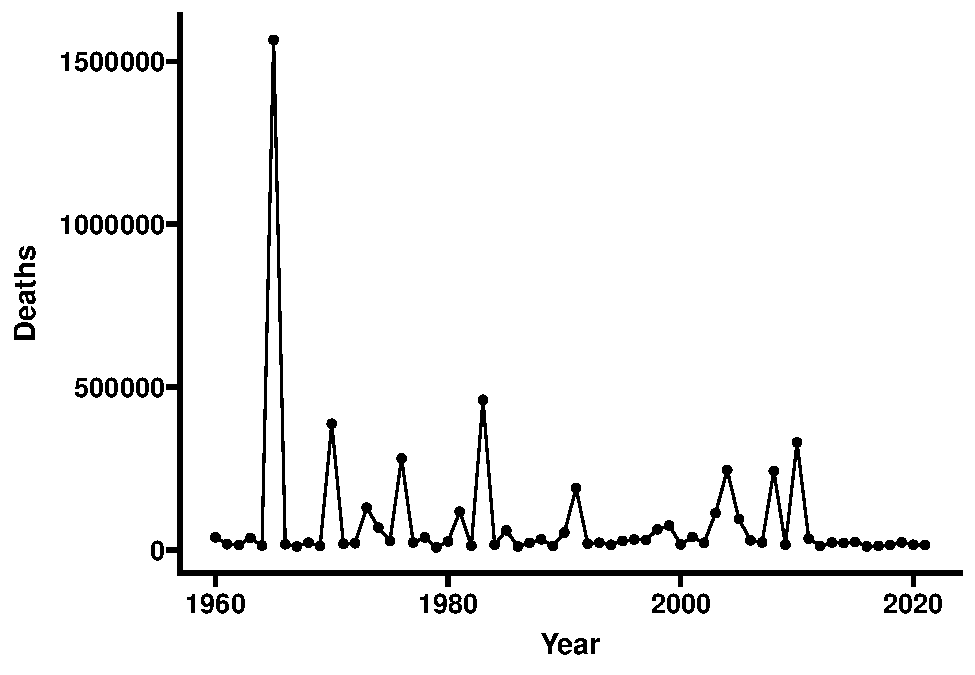
\includegraphics[width=1\linewidth]{disaster_effects_files/figure-latex/plot-deaths-1} 

}

\caption{Total number of deaths from natural disasters by year}\label{fig:plot-deaths}
\end{figure}

\hypertarget{methods}{%
\section{Methods}\label{methods}}

Analyses were conducted using the R Statistical language (4.2.2) \autocite{R-base} and Visual Studio Code (1.75.0-insiders) on Windows 11 x64 (build 22623) with an Intel Core-i5-4690K CPU with 24GB RAM, using the packages lme4 \autocite{R-lme4}, lmerTest \autocite{R-lmerTest}, easystats \autocite{R-easystats} and tidyverse \autocite{R-tidyverse}.

\hypertarget{data-acquisition-and-processing}{%
\subsubsection{Data Acquisition and Processing~}\label{data-acquisition-and-processing}}

Population data were sourced from United Nations World Population Prospects \autocite{unitednationsWorldPopulationProspects2022}. Economic data were sourced from the World Bank World Development Indicators \autocite{worldbankWorldDevelopmentIndicators2022}. Disaster data were based on the EM-DAT database \autocite{cred/uclouvainEMDATInternationalDisaster2023}.

Disaster, population and economic data sources were combined using the ISO country code as the identifying key. Population data from 1950-2021 were joined with projected data for 2022-2100, and subsequently data were restricted to the years ranging from 1960-2022. Economic variables containing ``..'' were converted to NA values for use in analysis, and irrelevant variables were removed, and information regarding disaster type, deaths, country, number of people affected, population, gdp, and government expendature on the military, education and healthcare were selected for inclusion. Percentage values for the number of people affected and number of deaths were calculated by dividing the population at the time of the disaster with the total deaths and total affected values.\footnote{Complete preprocessing script is available at \url{https://github.com/Digital-Methods-HASS/au662726_Ring_Luke/blob/main/exam/scripts/01_import_collate_source_data.R}} A total of 14,920 events were included from the data, and before analysis, 134 events from disaster types with less than 100 occurrences were excluded, removing Fog, Mass movement (dry), Insect infestation, Impact, Animal accident and Glacial lake outburst, leaving a remaining total 14,786 events for analysis.

\hypertarget{models}{%
\subsubsection{Models}\label{models}}

Two main models were used to analyse the possibility of predicting the scale of effects from natural disasters. Model 1 uses the scaled value from the percentage of GDP spent on education as a predictor variable and uses the number of deaths as a percentage of the population at the time of the disaster as the outcome variable, allowing for varying intercepts based on the type of natural disaster.

Model 2 uses the scaled value from the percentage of the population living in rural areas as a predictor variable and uses the number of affected people as a percentage of the population at the time of the disaster as the outcome variable, allowing for varying intercepts based on the type of natural disaster.

\hypertarget{results}{%
\section{Results}\label{results}}

\hypertarget{empircal-results}{%
\subsection{Empircal results}\label{empircal-results}}

\hypertarget{model-1}{%
\subsubsection{Model 1}\label{model-1}}

A linear mixed model was fitted (estimated using REML and nloptwrap optimizer) to predict deaths\_pct with edu\_exp\_pct\_gdp (formula: deaths\_pct \textasciitilde{} scale(edu\_exp\_pct\_gdp)). The model included disaster\_type as
random effect (formula: \textasciitilde1 \textbar{} disaster\_type). The model's total explanatory power is substantial (conditional R2 = 0.70) and the part related to the fixed effects alone (marginal R2) is of 2.03e-04. The
model's intercept, corresponding to edu\_exp\_pct\_gdp = 0, is at 0.08 (95\% CI {[}-0.05, 0.21{]}, t(5989) = 1.16, p = 0.246). Within this model:

\begin{itemize}
\tightlist
\item
  The effect of edu exp pct gdp is statistically significant and negative (beta = -3.59e-03, 95\% CI {[}-7.12e-03, -7.05e-05{]}, t(5989) = -2.00, p = 0.046; Std. beta = -0.03, 95\% CI {[}-0.05, -4.92e-04{]})
\end{itemize}

Standardized parameters were obtained by fitting the model on a standardized version of the dataset. 95\% Confidence Intervals (CIs) and p-values were computed using a Wald t-distribution approximation.

\hypertarget{model-2}{%
\subsubsection{Model 2}\label{model-2}}

A linear mixed model was fitted (estimated using REML and nloptwrap optimizer) to predict affected\_pct with rural\_population\_pct (formula: affected\_pct \textasciitilde{} scale(rural\_population\_pct)). The model included
disaster\_type as random effect (formula: \textasciitilde1 \textbar{} disaster\_type). The model's total explanatory power is substantial (conditional R2 = 0.32) and the part related to the fixed effects alone (marginal R2) is of
3.68e-03. The model's intercept, corresponding to rural\_population\_pct = 0, is at 21.90 (95\% CI {[}-7.32, 51.13{]}, t(11250) = 1.47, p = 0.142). Within this model:

\begin{itemize}
\tightlist
\item
  The effect of rural population pct is statistically significant and positive (beta = 4.90, 95\% CI {[}3.62, 6.19{]}, t(11250) = 7.48, p \textless{} .001; Std. beta = 0.07, 95\% CI {[}0.05, 0.08{]})
\end{itemize}

Standardized parameters were obtained by fitting the model on a standardized version of the dataset. 95\% Confidence Intervals (CIs) and p-values were computed using a Wald t-distribution approximation.

\hypertarget{discussion}{%
\section{Discussion}\label{discussion}}

While there results indicate a correlation between the predictor variables, it's difficult to draw conclusions from them because there are many confounding factors when trying to analyse the effects of natural disasters. Obviously, geographic location plays a role, as living on faultlines will increase the likelyhood of earthquakes. The same can be said for hurricanes, tsunamis and other natural disasters. The same can be said for the economic situation of a country, as a country with a higher GDP will have more resources to deal with disasters, and a country with a lower GDP will have less resources to deal with disasters.

Furthermore, there have been criticisms of the EM-DAT database containing biases in data prior to 1995 \autocite{panwarDisasterDamageRecords2020}. As such, further analyses may include data from other sources to compare the results.

Although the results are not conclusive, they do indicate that there is a correlation between the predictor variables and the outcome variables, and that further analysis is required to determine the effects of natural disasters on the population.
There are many possible further areas of investigation with data that is already available, and could potentially yield valuable results for informing future governmnet policy, and suggesting the most effective areas to provide aid to.
\balance
\clearpage


\printbibliography[title=References]

\end{document}
